%  sample input file for using the CSLI.cls LaTeX class

%  next 2 lines pull in the CSLI.cls file, put options between []
\documentclass[nocover]            % options: coveronly, nocover
{CSLI}                       %   plus standard article class options


\usepackage[
bookmarks=true,
bookmarksnumbered=false,  % true means bookmarks in
% left window are numbered
bookmarksopen=false,      % true means only level 1
% are displayed.
]{hyperref}

\usepackage{multirow}
\usepackage{titlesec}
\setcounter{secnumdepth}{4}

\graphicspath{ {images/} }

\usepackage{tikz-qtree}
\usepackage{mdframed}




%list separation
\setlist{nolistsep}
\setlist{noitemsep}

\abstract{CySat, Iowa State University's CubeSat program, is seeking a review of the educational and scientific merit of the CySat I mission. The review is for the purpose of applying to NASA's CubeSat Launch Initiative. This review will address the quality and benefits of the CySat I mission and it's relevance to NASA's Strategic Plan and Education Strategic Coordination Framework.}   % suggested 200 words


%%%%%%%%%%%%%%%%%%%%%%%
\begin{document}
\newpage
\tableofcontents

\pdfbookmark[2]{Contents}{table}


\newpage
\section{Introduction}
CySat is designing a nanosatellite platform in accordance with the CubeSat standard set forth by California Polytechnic University and Stanford University. The CubeSat program offers educational institutions, like Iowa State, the opportunity to design a space worthy satellite for a relatively low cost. The primary educational objective of CySat is the establishment of a small satellite program at Iowa State that allows the opportunity for students to apply their knowledge and coursework to a real astronautics project. CySat pulls students from a number of the Engineering Departments to foster an interdisciplinary environment within the College of Engineering and accomplish complex missions requiring multiple areas of expertise. Students have the opportunity to design a system and mission for a small satellite from concept to flight. CySat teaches it's members how to function within a multidisciplinary engineering team and gives them access to established industry and NASA contacts.  CySat provides a unique educational experience which helps prepare students for working in the space industry.
\subsection{Project Overview}
CySat falls under the umbrella of Iowa State's College of Engineering Make to Innovate organization (M:2:I). M:2:I is devoted to giving students the opportunity to submit proposals for engineering projects and supplying resources to help students independently fulfill those goals. Students in M:2:I receive academic credit for their contributions to their projects. CySat is an ongoing M:2:I project that has a strong history of support and backing from the department. CySat adheres to M:2:I's goals of providing further hands on educational experience for undergraduates outside of classes.\\
CySat is provided a faculty academic advisor by M:2:I and has acquired the assistance of three technical advisors, one at NASA's Johnson Space Center and two at Boeing. CySat is student run and composed of six individual teams that each focus on a specific subsystem of the satellite. CySat has developed this project structure to increase the efficiency of the teams design process and provide members with an authentic representation of space missions in industry.

\subsubsection{Project Goals}
The overall goals for CySat have been the driving force behind all design considerations and operational plans. The following were developed jointly between CySat and the team's academic advisors. 
\begin{enumerate}
\item Serve as a catalyst for the small satellite program at Iowa State University
\item Develop a baseline, modular design for future CubeSat missions
\item Demonstrate the functionality of CubeSat's for asteroid surveying
\end{enumerate}

\subsubsection{Project Structure}

\begin{figure}[H]
\centering
\tikzset{edge from parent/.style=
{draw, edge from parent path={(\tikzparentnode.south)
-- +(0,-8pt)
-| (\tikzchildnode)}},
blank/.style={draw=none},
level distance=60pt}


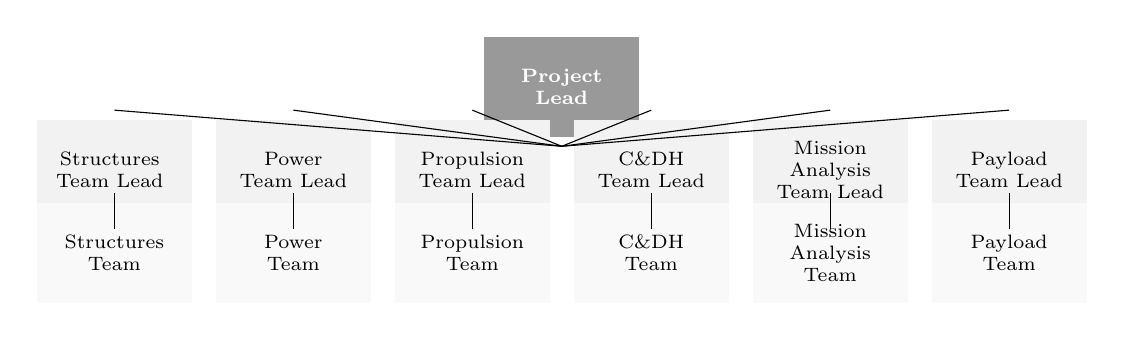
\begin{tikzpicture}[every tree node/.style={align=center}]
\Tree 
 [ .{\colorbox{gray!80}{\makebox(50,30){\parbox{4em}{\centering\scriptsize\textcolor{white}{\textbf{Project\\Lead}}}}}}
     [ .{\colorbox{gray!10}{\makebox(50,30){\parbox{4em}{\centering\scriptsize Structures Team Lead} }}}
       [ .{\colorbox{gray!5}{\makebox(50,30){\parbox{4em}{\centering\scriptsize Structures Team}}}} ]]
     [ .{\colorbox{gray!10}{\makebox(50,30){\parbox{4em}{\centering\scriptsize Power Team Lead}}}} 
       [ .{\colorbox{gray!5}{\makebox(50,30){\parbox{4em}{\centering\scriptsize Power Team}}}} ]]
     [ .{\colorbox{gray!10}{\makebox(50,30){\parbox{4em}{\centering\scriptsize Propulsion Team Lead}}}}
       [ .{\colorbox{gray!5}{\makebox(50,30){\parbox{4em}{\centering\scriptsize Propulsion Team}}}} ]]
     [ .{\colorbox{gray!10}{\makebox(50,30){\parbox{4em}{\centering\scriptsize C\&DH Team Lead}}}}
       [ .{\colorbox{gray!5}{\makebox(50,30){\parbox{4em}{\centering\scriptsize C\&DH Team}}}} ] ]
     [ .{\colorbox{gray!10}{\makebox(50,30){\parbox{4em}{\centering\scriptsize Mission Analysis Team Lead}}}} 
       [ .{\colorbox{gray!5}{\makebox(50,30){\parbox{4em}{\centering\scriptsize Mission Analysis Team}}}} ]]
     [ .{\colorbox{gray!10}{\makebox(50,30){\parbox{4em}{\centering\scriptsize Payload Team Lead}}}} 
       [ .{\colorbox{gray!5}{\makebox(50,30){\parbox{4em}{\centering\scriptsize Payload Team}}}} ]]] 
\end{tikzpicture}
\caption{CySat Team Hierarchy}
\end{figure}
\paragraph{Teams}
\textbf{Structures Team:}\\
The Structures Team is responsible for the structural design of the satellite. The team is working with computer aided design (CAD) software in order to model the satellite's configurations. Structures is designing mechanical testing procedures and will oversee the satellite's integration in order to  ensure it is compliant with the structural design.\\\\
\textbf{Power Team:}\\
The Power Team controls power generation, storage, and management for the satellite. The Power Team is currently finalizing the design of the solar arrays, and assisting the Propulsion Team in the implementation of stabilization.\\\\ 
\textbf{Propulsion Team:}\\
The Propulsion Team is currently performing research to find the ideal propulsion system to use for future asteroid missions. With current information, the team is focusing on electric engines and cold gas thrusters. Propulsion is also assisting Power in the implementation of stabilization.\\\\
\textbf{Communications \& Data Handling Team (C\&DH):}\\
The C\&DH team's focus is on the terrestrial and vehicle infrastructure and software. The team is designing and fabricating the flight computer and creating a robust, automated ground station and a beta mission control application. C\&DH is preparing for the finalization of the onboard radio band, mode and hardware along with data serialization format and telemetry processing.\\\\
\textbf{Mission Analysis Team:}\\
Mission Analysis is responsible for application of orbital mechanics to practical problems concerning the motion the satellite. Additionally, the team is responsible for designing the mission architecture and assessing the feasibility of comprehensive mission designs.\\\\
\textbf{Payload Team:}\\
The Payload Team will lead the scientific justification, acquisition and development of mission specific instrumentation. The Payload Team is working on the development of an asteroid-surveying payload, which will detect valuable resources within an asteroid and provide estimates of the location and quantity of the material.

\subsection{Mission Objectives}
CySat's current primary scientific objective is to demonstrate that CubeSats can be used as effective tools for the asteroid mining industry. CySat is developing a payload for asteroid surveying. CySat's first mission, CySat I, will be a proof-of-concept flown in Low Earth Orbit (LEO). CySat I will demonstrate the state-of-the-art communications and radar payload, the functionality of the satellite platform, and CySat's operational readiness. CySat I's payload will map the target's density and collect absorption spectrum's to determine the target's composition. CySat's CubeSat platform has been designed to be adaptable for different payload configurations, this will allow CySat to repurpose the platform for future missions.

\section{Design Factors}
Because of the recent surge in private industry support for CubeSats, CySat has been able to capitalize on recent commercial off-the-shelf (COTS) components to minimize design time and risk. The design team focused on COTS components due to several factors: flight heritage, short development time, and out of box functionality. Key components will be purchased commercially to decrease risk while some electronics will be developed in-house to increase efficiency. This system has allowed CySat to develop complex mission specific components in-house due to the increased flexibility of the commercial systems.
\subsection{Satellite Component Evaluation Criteria}
\textbf{Mass:} Pursuant to CubeSat specifications, special considerations were made to select and design components that would keep the system under the 4.0 Kg mass requirement.\\ 
\\\textbf{Volume:} Ensuring that components would not consume too much of the 10 x 10 x 30 cm cube, and building in allowances for a diverse range of mission specific payloads. \\
\\\textbf{Cost:} Due to the current fiscal situations of most state funded institutions, some high dollar amount components will be fabricated in house. \\
\\\textbf{Flight Heritage:} Knowing that components had successfully worked in the space environment was of great importance. This can be seen with the selection of COTS components.\\ 
\subsection{Design Restrictions}
The CubeSat team developed several design restrictions to guide and optimize the design early on. Since the payload will require substantial resources from the spacecraft, the design goal was to provide a robust platform with enough features to allow the spacecraft to operate beyond LEO. This strategy has produced a satellite platform which can be easily adapted for future collaborations with small businesses and other universities. 
\begin{enumerate}
\item The spacecraft shall conform to the 3U CubeSat standard
\item Spacecraft subsystems should be as simplistic as possible to reduce failure points 
\item Non-deployable solar arrays will be manufactured in house due to design needs and cost restrictions
\item COTS components will be used when possible to limit risk. Custom, mission optimized, electronics will be designed to increase efficiency
\end{enumerate}

\section{Science Implementation}
To accomplish the scientific mission objectives, CySat has developed a state of the art communications and radar payload. CySat is actively collaborating with the Caterpillar \& Iowa State Space Mining Operations team (CISSMO) to identify the relevant information which can be gained from prospecting an asteroid. CySat I's scientific payload will be based upon an integrated software defined radar for density and spatial mapping and an infrared spectrometer for collecting composition data. CySat I will fly the block I version of the payload which will serve as a risk-reduction pathfinder build of the software radio architecture designed for the mapping and prospecting of asteroids.
\subsection{Radar}
\subsubsection{Science Justification}
The CySat Mapping Radar (CMR) will serve as the primary scientific instrument and provide both a geodetic datum to correlate other instrumentation to, as well as returning data on the density and geological features of the target. Leveraging the flexibility of the software defined radio (SDR), the radar system is designed to provide spatial and density mapping by interrogating with different bands of radio energy as required. The application of reconfigurable hardware makes for an efficient and upgradeable platform to run radar across the spectrum as needed. By mapping data from all instruments aboard the satellite to a master spatial/density map, a total sense of the asteroid's composition and excavation viability can be assessed.
\subsubsection{Principles of Operation}
Underpinning the system is a SDR. By moving components of a traditional radio signal pipeline out of the hardware domain and into digital signal processing (DSP), a lighter and more flexible radio system can be created. All these desirable characteristic not only reduce energy and space usage on board the satellite, but also enable the SDR to function as the primary communications system, as well an integral component of the instrumentation payload.\newline
\indent Once in orbit of the target, the radar will operate as a synthetic aperture radar (SAR) where the relative motion of the satellite acts to increase apparent size of the antenna. This effect allows for successive passes of the target to act in place of a well matched antenna to regain lost accuracy and permits the selection of an antenna better suited for the chassis of the satellite.
\subsubsection{Implementation}
The CySat I mission will fly the CMR Block I. To accomplish this goal, the CMR is a synthetic aperture radar capable software defined radio for planetary radio imaging. The benefits of SDR for this experimental platform such as the flexibility in application (utilization for communications as well as radio navigation and radar mapping in multiple RF bands), reduction in system complexity (over having separate radio instruments for each function), and ease of manufacture by the reduced component count were key in selecting this approach. The intrinsic reprogrammability of the system will enable the CySat Payload Development Team to undertake progressive radar experiments with the CMR Block I until the satellite reaches end-of-life, including missions developed during flight with data from initial check-out.\\
\subsection{Spectrometer}
\subsubsection{Science Justification}
Infrared spectroscopy is used for determining the chemical composition of molecules. Infrared spectrometers have been used in many applications such as atmospheric observation, forensic analysis, and analysis of solid samples. CySat will use this technique to determine the chemical composition of an asteroid and search for minerals, metals and ices, which would be valuable resources for mining.
\subsubsection{Principles of Operation}
Infrared spectroscopy is the study of the interaction of electromagnetic radiation and matter, in the infrared range. Infrared spectroscopy provides access to quantifiable chemical information about the target. An infrared spectrometer is used to detect the light reflected by the target. When compared to the light emitted, a spectrum of the light absorbed can be produced. An infrared spectrum is a plot of the absorbance or transmittance of infrared light as a function of its wavelength or frequency. Different wavelengths of light are absorbed by different types of bonds and correspond to vibrations unique to the molecule. This allows the molecular structure and chemical composition of the target to be determined based on the infrared spectrum.
\subsubsection{Implementation}
CySat I will be flying the CySat Infrared Spectrometer Block I, which will consist of a COTS infrared spectrometer, the Argus 1000. The Argus 1000 is a miniature infrared spectrometer, designed for nanosatellites, with a proven flight heritage on multiple CubeSats. The Argus 1000, developed by researchers at York University, is currently commercially available and is the primary option CySat is considering for the surveying payload. The Argus 1000 was flown on the CanX-2 CubeSat, a mission by UTIAS/SFL (University of Toronto, Institute for Aerospace Studies/Space Flight Laboratory), and was designed to collect atmospheric spectra. The Argus 1000 has also been flown successfully on SRMSAT of Sri Ramaswamy Memorial University in Chennai. SRMSATs primary mission was a demonstration of the satellite platform and secondary was the operation of the Argus 1000 spectrometer for monitoring greenhouse gasses in the atmosphere. Both of these missions will serve as models for CySat's implementation of the Argus 1000 as the CySat Infrared Spectrometer Block I. The Argus 1000's small form factor, will fit easily within the volume allocated for the payload. The CySat Infrared Spectrometer Block I will provide the necessary operational experience for the team to develop a Block 2 Spectrometer that can reach the spectral ranges required to detect minerals, heavy metals, and ices.

\section{Schedule}
CySat is currently aiming for a completed satellite by May 2018. To support this, the following schedule has been developed.
\begin{table}[H]
\centering
\caption{CySat I Development Schedule}
\begin{tabular}{| l | l | l |}
\arrayrulecolor{white}
\hline
\rowcolor{gray!80}
\textcolor{white}{\textbf{Task}} & \textcolor{white}{\textbf{Semester(s)}} & \textcolor{white}{\textbf{Dates}} \\ \hline
\rowcolor{gray!10}
Design Finalization & Fall 2016 - Spring 2017& August 22nd - May 6th  \\ \hline
\rowcolor{gray!5}
Fabrication & Spring - Fall 2017 & January 9th - December 16th  \\ \hline
\rowcolor{gray!10}
Testing & Spring 2018 & January 8th - May 5th   \\ \hline
\rowcolor{gray!5}
Delivery & Summer 2018 & May 15th \\ \hline
\end{tabular}
\end{table}

\section{Budget}
\subsection{Funding Sources}
CySat has been able to work with many organizations over the last year to secure sources of monetary funding and in-kind donations. The main suppliers of funding have been Iowa Space Grant Consortium, NASA JSC, Boeing, Rockwell Collins, and Iowa State University's Electrical Engineering and Aerospace Engineering departments. Through continued dialogue, funding has been guaranteed to continue through the next two years until satellite completion. CySat is also in the process of obtaining in-kind donations to minimize cost for testing the satellite structure and acquiring the Argus 1000 Spectrometer. The following budget has been developed as a conservative estimate of the total project cost.
\subsection{Budget Component Breakdown}
\begin{table}[H]
\centering
\caption{Budget Component Breakdown}
\begin{tabular}{| l | p{5cm} | r |}
\arrayrulecolor{white}
\hline
\rowcolor{gray!80}
\textcolor{white}{\textbf{Subsystem}} & \textcolor{white}{\textbf{Item(s)}} &  \textcolor{white}{\textbf{Cost (\$)}} \\ \hline
\rowcolor{gray!10}
Structures & Manufacturing&1,000 \\
\rowcolor{gray!10}
 &Mounting hardware &500 \\ \hline
\rowcolor{gray!5}
Power & Electronic power system & 9,000\\
\rowcolor{gray!5}
& Solar array side panels &15,000 \\
\rowcolor{gray!5}
& Deployable solar array & 28,000\\ \hline
\rowcolor{gray!10}
Stabilization & Active stabilization&15,000 \\ 
\rowcolor{gray!10}
&Passive stabilization &7,000 \\ \hline
\rowcolor{gray!5}
C\&DH& Flight Computer &1,050\\
\rowcolor{gray!5}
& Radio board& 8,600\\ \hline
\rowcolor{gray!10}
Payload & CMR block I &2,500 \\ 
\rowcolor{gray!10}
& Argus 1000 spectrometer &50,000 \\
\rowcolor{gray!10}
& Payload antenna & 800\\\hline
\rowcolor{gray!5}
 &  & Total: 138,450\\ \hline
\end{tabular}
\end{table}

\section{Relevance to NASA}
CySat's educational and mission objectives align with multiple NASA Strategic Goals (Appendix B) and Education Outcome Objectives (Appendix A) which have been identified in the sections below.
\subsection{Strategic Goals}

\subsubsection{Objective 2.3}
\begin{table}[H]
\centering
\begin{tabular}{| p{\textwidth} |}
\arrayrulecolor{white}
\hline
\rowcolor{gray!80}
\textcolor{white}{\textbf{Strategic Objective 2.3: }} \\ \hline
\rowcolor{gray!10}
Optimize Agency technology investments, foster open innovation, and facilitate technology infusion, ensuring the greatest national benefit.\\ \hline
\end{tabular}
\end{table}
CySat has a history of collaboration and technology transfer and all of CySat's Designs will be made publicly available after successful completion of the mission. CySat is currently collaborating with other projects at Iowa Sate such as the M:2:I High Altitude Balloon Experiments in Technology team (HABET), to perform high altitude balloon tests for payload components, and with the Caterpillar \& Iowa State Space Mining Operation (CISSMO), a project which could realistically benefit from CySat's asteroid surveying mission. In the past, CySat has collaborated with Softronics Ltd. and the University of North Dakota on two different past projects. CySat completed the design of a 1U CubeSat platform which was adapted for the two different outsourced payloads. Neither satellite flew as neither payload was completed. CySat plans to return to this collaborative mission model after completing the 3U CubeSat platform and acquiring flight heritage. CySat hopes to encourage involvement in the space industry by providing a robust and adaptable space vehicle platform for scientific payloads developed by small business and universities.\\  
\indent CySat has focused on delivering the following benefits to encourage involvement and innovation in the space industry and facilitate technology transfer: 
\begin{enumerate}
\item{Developing relationships and fostering collaborations in industry and academia}
\item{Sharing research, designs, and information with the public to benefit the scientific and small satellite communities}
\item{Development of an adaptable 3U CubSat platform for providing space vehicle services for innovative outsourced missions}
\item{Completion of an asteroid surveying payload to help support space mining efforts and advance the developments of software defined radar for space applications}
\end{enumerate} 

\subsubsection{Objective 2.4}

\begin{table}[H]
\centering
\begin{tabular}{| p{\textwidth} |}
\arrayrulecolor{white}
\hline
\rowcolor{gray!80}
\textcolor{white}{\textbf{Strategic Objective 2.4: }} \\ \hline
\rowcolor{gray!10}
Advance the Nation's STEM education and workforce pipeline by working collaboratively with other agencies to engage students, teachers, and faculty in NASA's missions and unique assets.\\ \hline
\end{tabular}
\end{table}
As described in section 6.1.1, CySat has a long history of collaboration. CySat and it's advisors meet on a biweekly basis to evaluate the state of the project. This provides members with direct contact and input from CySat's technical advisor at NASA JSC, Lee Graham. CySat hopes to continue developing this relationship and fly NASA payloads on future missions. These collaborations not only provide beneficial information and resources for the project they also teach the student members how to manage professional relationships and facilitate direct contact with professionals in industry. CySat's mission has been designed not only to benefit private space mining efforts but also to align with NASA's goals. As stated in NASA's Strategic Plan, NASA's has a bold new initiative to capture and explore an asteroid and is currently undertaking detailed examination of NEA's (Appendix B: NASA's Strategic Plan). CySat's asteroid surveying payload would provide valuable information for any asteroid exploration mission. CySat's primary option for acquiring a launch vehicle is through the NASA CubeSat Launch Initiative (CSLI). CySat's CubeSat platform has been designed to NASA's specifications to ensure the projects ability to take advantage of this initiative and use NASA's unique launch assets. CySat provides an opportunity for students to receive credit while directly collaborating with NASA and designing systems directly related to NASA's missions and goals.\\
\indent CySat has identified the following benefits which provide students with access to industry and enables them to engage in NASA's missions while receiving an education:
\begin{enumerate}
\item{Developing relationships and fostering collaborations in industry and academia}
\item{Direct collaboration with a technical advisor at NASA}
\item{Development of an asteroid surveying payload with direct benefits to NASA's ambitious goals regarding the exploration of asteroids}
\item{All systems must be designed to NASA's specifications to benefit from NASA's launch initiatives}
\end {enumerate}

\subsection{Education Outcome Objectives}

\begin{table}[H]
\centering
\begin{tabular}{| p{\textwidth} |}
\arrayrulecolor{white}
\hline
\rowcolor{gray!80}
\textcolor{white}{\textbf{Educational Outcome Objective 1.3: Student Involvement, Higher Education (Educate) }} \\ \hline
\rowcolor{gray!10}
Provide opportunities for groups of post-secondary students to engage in authentic NASA-related mission-based research and development activities.\\ \hline
\end{tabular}
\end{table} 

\begin{table}[H]
\centering
\begin{tabular}{| p{\textwidth} |}
\arrayrulecolor{white}
\hline
\rowcolor{gray!80}
\textcolor{white}{\textbf{Educational Outcome Objective 1.4: Course Development (Educate)}} \\ \hline
\rowcolor{gray!10}
Develop NASA-related course resources for integration into STEM disciplines.\\ \hline
\end{tabular}
\end{table} 

\begin{table}[H]
\centering
\begin{tabular}{| p{\textwidth} |}
\arrayrulecolor{white}
\hline
\rowcolor{gray!80}
\textcolor{white}{\textbf{Educational Outcome Objective 1.5 Targeted Institution Research and Academic Infrastructure (Employ)}} \\ \hline
\rowcolor{gray!10}
Improve the ability of targeted institutions to compete for NASA research and development work.\\ \hline
\end{tabular}
\end{table}  

As stated in section 6.1.2, CySat's mission and systems are directly related to NASA's missions. CySat is working closely with NASA and is dependent on NASA resources to accomplish it's missions. Since CySat is a part of the M:2:I organization, students receive credit towards graduation for their contributions.  CySat provides a course option at Iowa State which is fundamentally related to NASA. CySat is preparing to take part in NASA's Cube Quest Challenge to secure a launch for CySat 2, the planned asteroid or lunar surveying mission which will begin after completion of CySat I. By applying for these initiatives and challenges, CySat's members gain experience delivering work which meets NASA's high standards of technical excellence. Acquiring successful flight heritage with CySat I will greatly improve CySat's likelihood of securing launch vehicles for future missions. By giving members access to NASA employees and other industry contacts, CySat enables students to build and expand their professional networks. CySat's project structure has been designed to give students an authentic industry experience by working on a project consisting of multidisciplinary teams and collaborating with NASA, private companies and other educational institutions. The unique experience members of CySat gain helps better prepare them for working in industry or with NASA.

CySat has identified the following benefits which enable students to receive an education through NASA related coursework and prepare students for employment:
\begin{enumerate}
\item{Train engineering team in planning, proposing, design, building, testing, launch, and operation of a satellite}
\item{Provide students with direct access to NASA employees and resources through collaborating with CySat's technical advisor at NASA JSC}
\item{Gives students academic credit for NASA-related projects towards their degrees}
\item{Gives students experience preparing technical and scientific reports for NASA research and development}
\item{Expose students to collaborative mission models and teach them to manage professional relationships}
\item{Foster an interdisciplinary environment within the College of Engineering at Iowa State University which gives students an authentic representation of space missions in industry}
\end{enumerate} 


\newpage
\section{Conclusion}
CySat plans to launch the first student built CubeSat from Iowa. CySat is working to establish a robust and modular platform for building low cost, low risk satellites on a short development timeline. The objective of CySat I's mission is a technology demonstration of the state-of-the-art communications and radar payload, the functionality of the satellite platform, and the satellite's operational capabilities. CySat's mission will showcase the diverse range of applications for low-cost small satellites and demonstrate their usefulness for surveying asteroids. In addition to readying students for work in the space industry, CySat is also working to further scientific study by increasing access to small satellites for small businesses in Iowa and student organizations. Through collaborations, this project would allow any interested group to test their space bound equipment using CySat's CubeSat platform, before investing resources in a full sized satellite. By completing CySat I's mission, the CySat team will obtain valuable flight heritage for the CySat I Platform and demonstrate that novel space missions are within scope of small businesses and universities.
\newpage
\section{Review Rubric}
CySat is asking for a review of merit for the NASA-CSLI proposal. In the review, the goals and objectives of the proposed investigation must be assessed to determine the scientific and educational quality of the investigation. The review must assess the overall alignment of the proposed investigation in addressing the objectives identified in the NASA Strategic Plan. The following questions have been drafted to help guide your analysis.\\
\begin{itemize}
\item[$\circ$]Is CySat providing students with opportunities to learn authentic NASA-related skills?\\
\item[$\circ$]Is CySat demonstrating its ability to design and implement novel space missions?\\
\item[$\circ$]Has CySat developed a robust asteroid surveying payload which will fulfill the missions objectives?\\
\item[$\circ$]Does the CySat I mission have scientific merit?\\
\item[$\circ$]Does the CySat I mission have educational merit?\\
\item[$\circ$]Is the CySat I mission relevant to NASA's Strategic Plan?\\
\item[$\circ$]Based on the scientific and educational merit of the mission, would you recommend that NASA provide a launch vehicle for CySat I?\\
\end{itemize}

\newpage
\appendix
\Appendix{NASA Education Strategic Coordination Framework: Education Outcome and Objective Hierarchy}
\includepdf[pages= {-} ]{NASA_ED.pdf}

\Appendix{NASA Strategic Plan}
\includepdf[pages= {5-46} ]{NASA_SP.pdf}


\end{document}

%%% Local Variables: 
%%% mode: latex
%%% TeX-master: t
%%% End: 
